\section{MUTE}

\begin{frame}{Architecture système de MUTE}
    \vspace{-0.5cm}
    \begin{figure}
        \resizebox{\textwidth}{!}{
            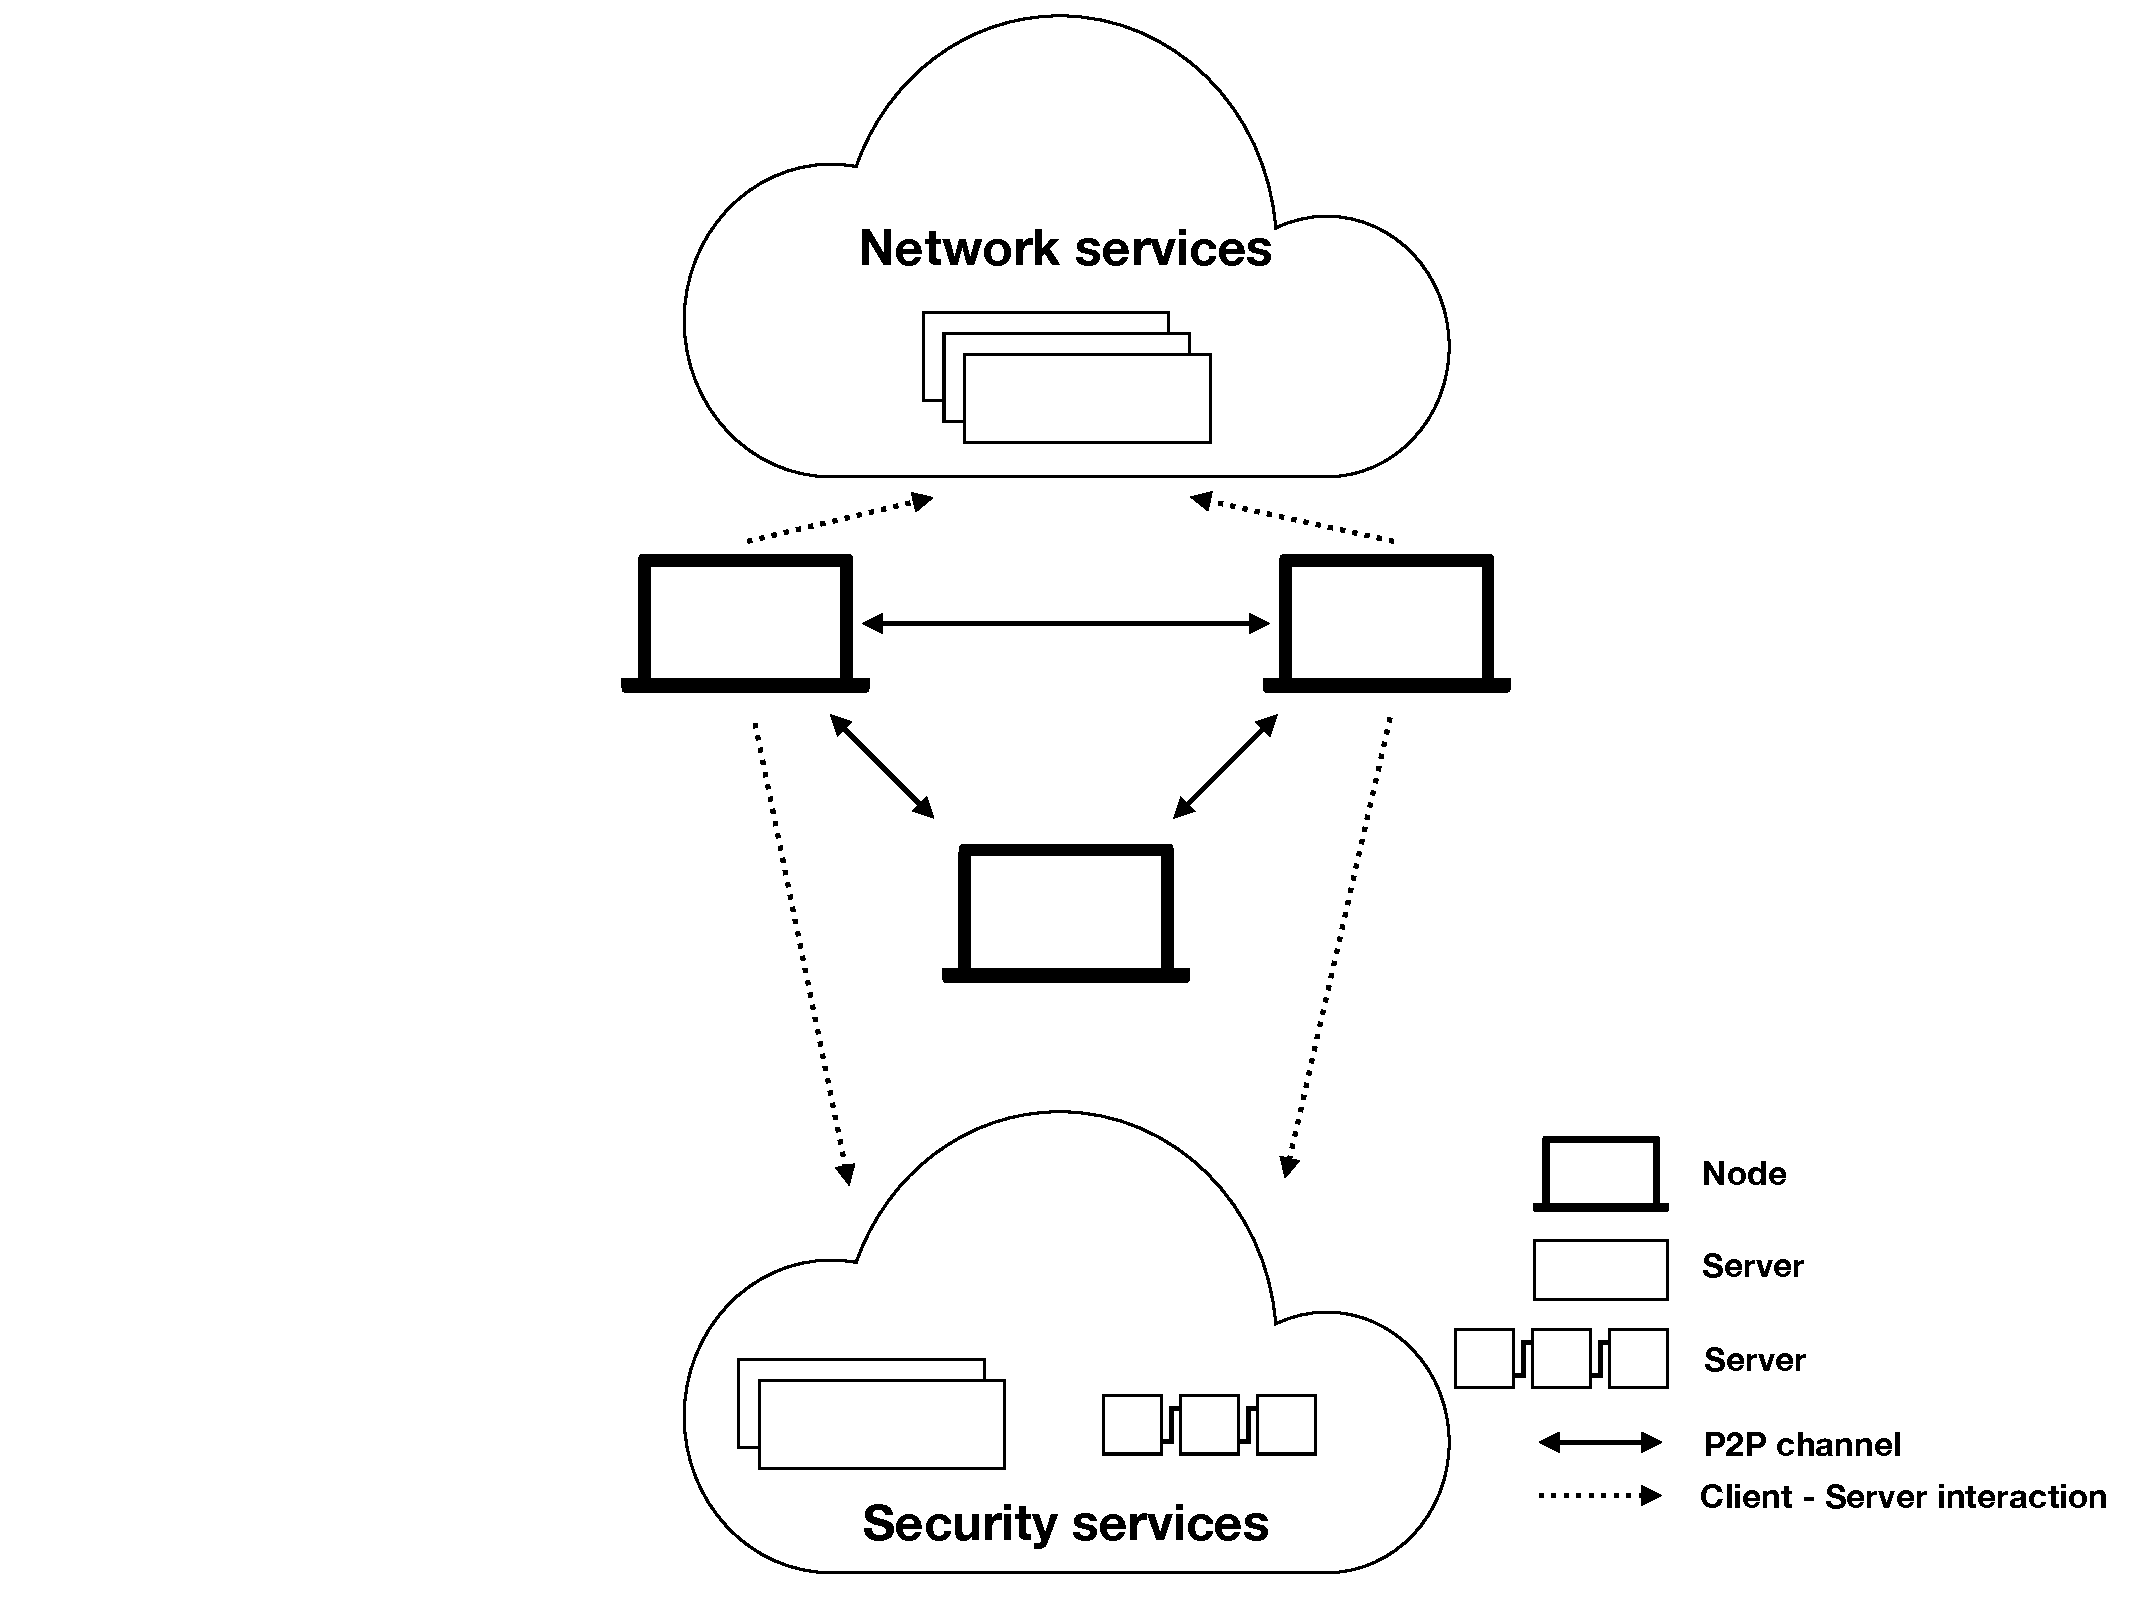
\includegraphics[page=1, trim=0cm 0cm 0cm 0cm, clip, width=.7\linewidth]{img/mute-figures.pdf}
            }
    \end{figure}
\end{frame}


\begin{frame}{Architecture logicielle de MUTE}
    \vspace{-0.5cm}
    \begin{figure}
        \resizebox{\textwidth}{!}{
            \includegraphics[page=2, trim=0cm 0cm 0cm 0cm, clip, width=.7\linewidth]{img/mute-figures.pdf}
        }
    \end{figure}
\end{frame}

\begin{frame}{Contributions}
    \metroset{block=transparent}
    \begin{block}{Document}
        \begin{itemize}
            \item Implémentation des CRDTs LogootSplit et RenamableLogootSplit
        \end{itemize}
    \end{block}

    \begin{block}{Operation Dependancies \& Anti-Entropy}
        \begin{itemize}
            \item Implémentation des modèles de livraison pour LogootSplit et RenamableLogootSplit
            \item Implémentation d'un mécanisme d'anti-entropie (détection et échange des opérations perdues)
        \end{itemize}
    \end{block}

    \begin{block}{Ingénierie logicielle}
        \begin{itemize}
            \item Mise en place des processus d'intégration continue et de livraison continue pour les librairies \texttt{mute-structs}\singlefootnote{\url{https://github.com/coast-team/mute-structs}} et \texttt{mute-core}\singlefootnote{\url{https://github.com/coast-team/mute-core}}
        \end{itemize}
    \end{block}
\end{frame}

\begin{frame}{Contributions - suite}
    \metroset{block=transparent}
    \begin{block}{Network}
        \begin{itemize}
            \item Supervision de la réalisation d'un \emph{Proof of Concept} basé sur l'utilisation d'un \emph{log-based message broker}
        \end{itemize}
    \end{block}

    \begin{block}{Collaborators}
        \begin{itemize}
            \item Supervision de l'adaptation et l'implémentation de SWIM, un protocole d'appartenance au réseau
        \end{itemize}
    \end{block}
\end{frame}
